\documentclass[12pt]{article}

\usepackage{amsmath}
\usepackage[authoryear,round]{natbib}
\usepackage{hyperref}



\textwidth=6.2in
\textheight=8.5in
\oddsidemargin=.1in
\evensidemargin=.1in
\headheight=-.3in

\newcommand{\scscst}{\scriptscriptstyle}
\newcommand{\scst}{\scriptstyle}
\newcommand{\Rfunction}[1]{{\texttt{#1()}}}
\newcommand{\Rmethod}[1]{{\texttt{#1}}}  
\newcommand{\Rclass}[1]{{\texttt{#1}}}
\newcommand{\Robject}[1]{{\texttt{#1}}}
\newcommand{\Rpackage}[1]{{\textit{#1}}}
\newcommand{\code}[1]{{\texttt{#1}}}
\bibliographystyle{plainnat}

\title{Outline: Analysis of High Throughput Flow Cytometry Data using \Rpackage{plateCore}}

%%%%%%%%%%%%%%%%%%%%%%%%%%%%%%%%%%%%%%%%%%%%%%%%%%%%%%%%%%%%%%%%%%%%%%%%%%%
\usepackage{/usr/local/lib64/R/share/texmf/Sweave}
\begin{document}
\maketitle

\clearpage
%%%%%%%%%%%%%%%%%%%%%%%%%%%%%%%%%%%%%%%%%%%%%%%%%%%%%%%%%%%%%%%%%%%%%%%%%%%%%%%%%%%%%%%%%%%%%%%%%%%%%%%%%%%%%%%%%%%%%%%%%%%%%%%%%%%
\section*{Abstract}
\subsection*{Background}
High throughput flow studies are often run in a 96 or 384-well plate format, with a number of different samples, 
controls, and antibodies-dye conjugates present on the plate. Analyzing the output from the cytometer requires keeping track of the contents
of each well, matching sample wells with control wells, gating each well/channel separately, making the appropriate plots, assessing quality, and
summarizing the results. This can be a monumental task using traditional point-and-click software packages, even when multiple instances are
deployed. We developed \Rpackage{plateCore} as an R/Bioconductor packaged to make processing and analysis of large, complex flow cytometry (FCM) datasets
easier. 

\subsection*{Methods}
\Rpackage{plateCore} was used to analyze the results from a BD FACS\texttrademark CAP screening experiment where 5 PBMC samples 
were assayed for 189 different human cell surface markers. 
This same dataset was also analyzed by a cytometry expert using FlowJo\texttrademark.

\subsection*{Results}
Positive markers identified using \Rpackage{plateCore} are in good agreement with those found using FlowJo\texttrademark analysis.

\subsection*{Conclusions}
\Rpackage{plateCore} provides a reproducible, objective platform for analyzing high throughput flow experiments. The R/Bioconductor 
implementation allows bioinformaticians and statisticians access to the data, which should further the development of automated
analysis methods.

\clearpage
%%%%%%%%%%%%%%%%%%%%%%%%%%%%%%%%%%%%%%%%%%%%%%%%%%%%%%%%%%%%%%%%%%%%%%%%%%%%%%%%%%%%%%%%%%%%%%%%%%%%%%%%%%%%%%%%%%%%%%%%%%%%%%%%%%
\section*{Introduction}
Analysis of flow cytometry high content screening (FC-HCS) experiments requires a systematic approach to
preprocessing, gating (i.e., filtering), and summarizing large amounts of data. Ideally these steps would be automated,
allowing analysis pipelines to be robust, objective, and match the high-throughput capacity of modern cytometers. 
Unfortunately, current approaches to FC-HCS analysis methods are semi-automated at best,
often requiring significant manual intervention to identify cells of interest and set the appropriate gates. 
Since the manual contribution is subjective and prone to error when working with large numbers of samples (ref Holden?), it
is desirable to develop programmatic approaches to process the data.

Flow cytometry packages available through the Bioconductor (ref) project provide an open analysis platform that
can be used by cytometrists, bioinformaticians, and statisticians to develop new analysis approaches that
enable automated processing. The \Rpackage{flowCore} (ref) package contains the framework for importing, transforming, gating, and
organizing raw flow cytometry data. \Rpackage{flowViz} (ref) supports sophisticated visualizations based on Trellis (ref?) displays. 
\Rpackage{flowClust} (ref) implements model-based clustering approaches for automated gating. \Rpackage{plateCore}
extends the \Rpackage{flowCore} and \Rpackage{flowViz} packages to work on \Robject{flowPlate} objects that represent
large flow datasets. The combination of these packages provides a set of freely available, flexible, and computationally efficient FC-HCS tools. 

An example of the progression from raw FCM data files to a completed \Rpackage{plateCore} analysis is shown in Figure~\ref{fig:analysis}.
List mode FCS files for a single plate are read into a \Robject{flowSet} using \Rpackage{flowCore}, and then a \Robject{flowPlate} is created by integrating
the plate annotation file with the \Robject{flowSet}. The \Robject{flowPlate} is then compensated, data quality is assessed, and gates
are set according to a negative control. These control gates are then applied to test wells to find cells that have specific staining
in channels of interest. Assuming that the automated gates do not require adjustment, and that there are no missing wells or other major problems,
the analysis of a single plate can be accomplished in 10-12 lines of code. While this same analysis can be performed relatively quickly in 
other flow cytometry software packages, it can be difficult to reproduce the gating decisions made by a single expert user.

In addition to subjective gating, the lack of a standard format for describing large flow experiments also
makes it difficult for anyone other than the original experimenter to replicate an analysis. 
The adoption of ACS specifications (ref) should make it easier to access metadata in future flow studies, but currently
this information is typically provided as a pictorial layout of a 96 well plate. 
Since the creation of \Robject{flowPlate} requires users to make a defined sample annotation file, plate layouts
can then be easily shared along with the raw FCS2.0/3.0 files. Also, this annotation can then be accessed
when working with \Robject{flowPlates} using either \Rpackage{flowCore} or \Rpackage{flowViz} functions.
The standard format for \Rpackage{plateCore} sample annotations provides a convenient way to manage the plate metadata
associated with complex FC-HCS experiments.

\Rpackage{plateCore} is not designed to be a GUI driven end-user tool, but rather to help develop a standardized platform for the analysis of FC-HCS data.
These analyses often represent a collaborative effort between cytometry experts who generate the data and the quantitative individuals who help
deal with the large volume information. In order for this collaboration to work, the cytometrists must have confidence in the
results of the automated analysis. To this point, we demonstrate the equality of our results to those produced by an expert
cytometrist using FlowJo\texttrademark.

%Since the layout of FC-HCS plates often changes from experiment
%to experiment, the annotation for each well needs to be customized for each
%\Rclass{flowPlate}. \Rpackage{plateCore} uses an approach that is very similar to the cell-based high throughput screening \Rpackage{cellHTS2} package (ref),
%where users must provide a \textit{plate configuration} file for each dataset. Once the cell level data has
%been analyzed in \Rpackage{plateCore}, the summary well information (i.e., percentage of positive cells and median
%signal intensities) can be imported into tools like \Rpackage{cellHTS2}, since FC-HCS experiments are just one 
%type of cell-based high throughput screens.

\begin{figure}
\centering
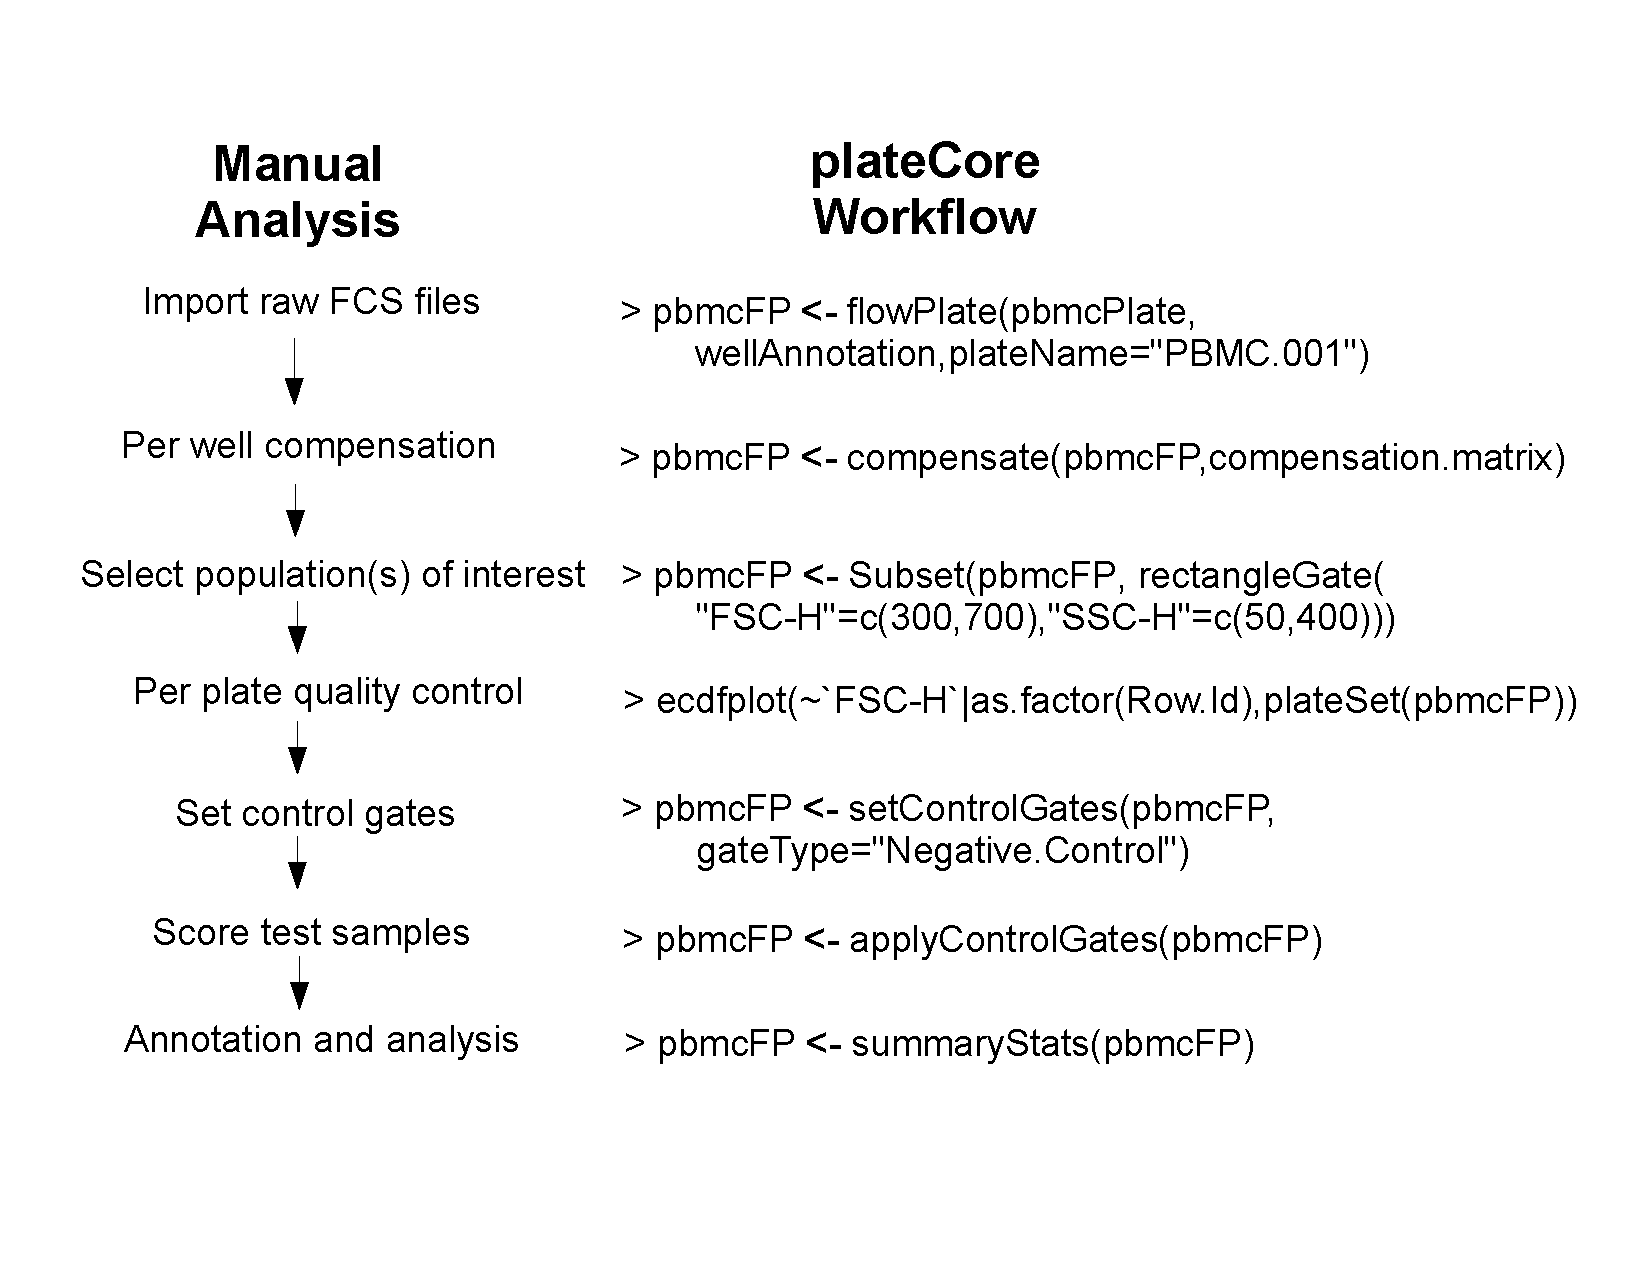
\includegraphics[width=7in,height=6in]{analysisSteps.pdf}
\caption{Typical plateCore workflow on the left, and examples of each step from a sample analysis are shown on the right.
Generating reports and plots is a multi-step that typically involves merging output from several plates, and the required
code is not shown here.
If necessary, the threshold control gates created automatically from \Rfunction{setControlGates} are adjusted based on input from flow experts. 
These new gates are established based on the gap between negative and positive test samples, whereas the automated
control gates were set using only negative control wells.}
\label{fig:analysis}
\end{figure}
 
%%%%%%%%%%%%%%%%%%%%%%%%%%%%%%%%%%%%%%%%%%%%%%%%%%%%%%%%%%%%%%%%%%%%%%%%%%%%%%%%%%%%%%%%%%%%%%%%%%%%%%%%%%%%%%%%%%%%%%%%%%%%%%%%%%%
\clearpage
\section*{Materials and Methods}
\subsection*{Data}

Get the flow group to describe how the samples were prepared?

The peripheral blood mononucleocyte (PBMC) data used in this study consists of 5 samples that were analyzed on 96-well plates
using BD FACS\texttrademark CAP (ref). On each plate, there are 189 different human cell surface antibody-dye conjugates that
are arrayed 3 per well (63 test wells), along with 30 isotype control wells and 3 unstained controls.
Test antibodies and isotypes are arrayed 3 per well, and the data was compensated
on the cytometer (BD FACSCalibur\texttrademark). The 189 antibodies were selected to provide a broad expression profile
for a large number of cell surface markers, including 103 proteins with GO annotation for receptor activity, 80
for immune response, and 55 for signal transduction. The raw data is available for download from http://www.ficcs.org as the
"plateData.tar.gz" file. The plate configuration is also included in the archive as \textit{maskPlateDesc.csv}, although
the antibody names have been masked. (Note: I need to update the description so it's compatible with the latest version of plateCore).

%%%%%%%%%%%%%%%%%%%%%%%%%%%%%%%%%%%%%%%%%%%%%%%%%%%%%%%%%%%%%%%%%%%%%%%%%%%%%%%%%%%%%%%%%%%%%%%%%%%%%%%%%%%%%%%%%%%%%%%%%%%%%%%%%%%
\subsection*{Analysis}

The goal of the PBMC FACS\texttrademark CAP study was to find the percentage of positive lymphocytes for each of the 189 different cell
surface markers. The raw data consists of a PBMC preparation, including lymphocytes, monocytes, red blood cells, and cellular 
debris. The first step is to filter the lymphocytes using a morphology gate in the forward (FSC) and side-scatter (SSC) channels. 
The quality of the data is then assessed by looking for fluidic events and making sure there are a sufficient number of cells in each
sample. Next the threshold between positive and negative cells are determined using the isoytpe controls, which provide a gross estimate
of non-specific binding in the primary antibodies. One-dimensional gates are created using using the isotype thresholds, and these
gates are applied to identify cells that are positively stained for each marker. An example of the code used to analyze an individual
plate is provided in this section.  The parameter settings for the other 4 plates are identical to the values shown here.

Ninety-six Flow Cytometry Standard (FCS) files, one for each well, are imported in R using \Rpackage{flowCore} to create a \Robject{flowSet}.
A \Robject{flowPlate} named platePBMCraw is then constructed by integrating the \textit{plate configuration} with the \Robject{flowSet}. 
The raw data is then visualized using \Rpackage{flowViz}, and a FSC-SSC \Robject{rectangleGate} is used to select lymphocytes (Figure ~\ref{fig:morphGate}).
A new \Robject{flowPlate} containing cells inside the \Robject{rectangleGate} is then made using \Rfunction{Subset}.
\begin{Schunk}
\begin{Sinput}
> platePBMC <- Subset(platePBMCraw,
+ 		rectangleGate("FSC-H"=c(300,700),"SSC-H"=c(50,400)))	
\end{Sinput}
\end{Schunk}

Quality control and quality assessment for large flow experiments is potentially more complex than the analysis itself. In this study, 
it would be desirable to verify that the 189 antibody-dye conjugates and their associated controls were aliquoted correctly into the correct wells, 
that the cytometer setting were not changed between plates, and that there were no fluidic events or shifts in fluorescent signals. Sophisticated tools for creating
quality reports for \Robject{flowSets} are available in \Rpackage{flowQ}, and the quality check functions can be customized for specific analyses.
Quality assessment in this example will focus on checking for fluidic events, which 
can cause a temporary shift in the cytometer detector readings.  Affected wells need
to be identified and either corrected or removed from the analysis. 
Fluidic events can often be identified by plotting the emprical cumulative density (ecdf) plots of FSC
values for each well, and looking for distributions shifted relative to other wells (Figure ~\ref{fig:fluidic}). Based on the ecdf
plots, several wells were further investigated by cytometry experts who determined that the shifts were in an acceptable range.

\begin{figure}
\centering
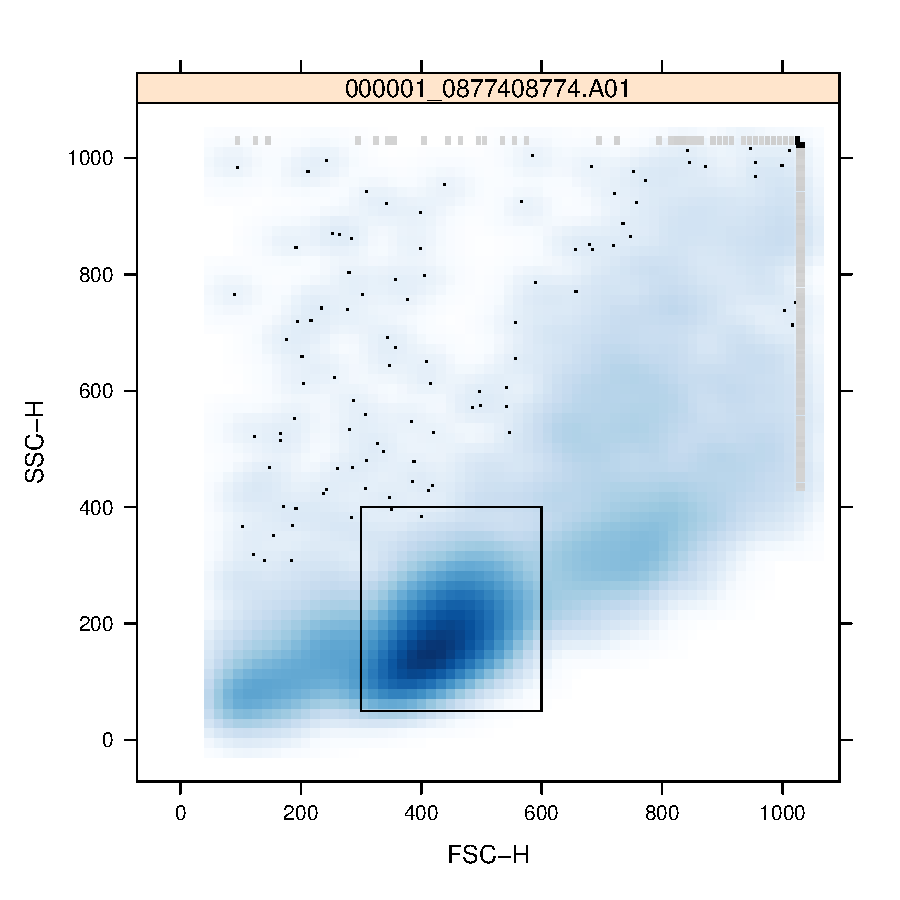
\includegraphics{outline-morphGate}
\caption{A \Rpackage{flowCore} rectangleGate used to select lymphocytes from PBMC data. The gate is displayed using the xyplot function from \Rpackage{flowViz}}
\label{fig:morphGate}
\end{figure}

\begin{figure}
\centering
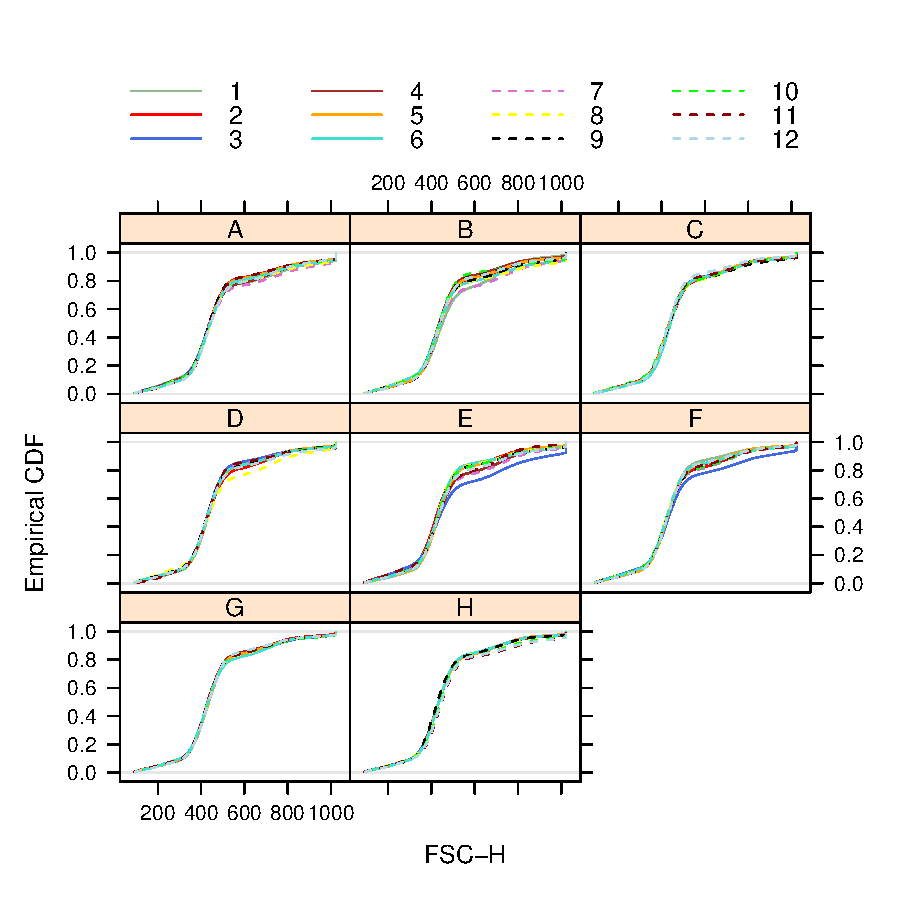
\includegraphics{outline-fluidic}
\caption{Empirical cumulative distribution function (ecdf) plots of FSC-H values for Rows A thru H. There are 12 columns in each row.
Fluidic events will often show up as a shift in the distribution of FSC-H values. 
Based on this plot wells E03 and F03 were manually checked, but the differences were not large enough to change fluorescence values.}
\label{fig:fluidic}
\end{figure}

\clearpage
Once the plate has passed quality control
checks, the next step is setting the control gate to establish the cutoff between positive and negative cells.
Ideally this expression threshold would be established using known positive and negative samples, but such information is
usually not available. Instead, the expression cutoff is generally set according to negative controls. 
For example, \Rpackage{plateCore} supports creating thresholds according to either unstained, unstimulated, isotype, 
or fluorescence minus one (FMO) controls. One-dimensional expression thresholds are initially set using
the setControlGates function. 
\begin{Schunk}
\begin{Sinput}
> platePBMC <- setControlGates(platePBMC,gateType="Negative.Control",numMads=6)
\end{Sinput}
\end{Schunk}
The "numMads" parameter sets the value of the control gate at 6 median absolute deviations (MADs) above 
the media fluorescence intensity (MFI) the control gate. An example of the isotype gating results for the isoytpe well A03 and its
associated test wells is shown in Figure~\ref{fig:isoGate}.
\Rpackage{flowCore} and \Rpackage{flowClust} potentially offer
more robust methods of establishing this threshold using kernel density approaches, but setting the
gate at 3 to 6 MADs on a linear scale (non-transformed) often works well in practice for screening quality experiments.

Once the Negative.Control gates have been created and applied, we can then use the \Rfunction{summaryStats} to calculate different
metrics of interest from the \Rclass{flowPlate}. Running \Rfunction{applyControlGates} and \Rfunction{summaryStats} on \Robject{platePBMC}, 
\begin{Schunk}
\begin{Sinput}
> platePBMC <- applyControlGates(platePBMC)
> platePBMC <- summaryStats(platePBMC)
\end{Sinput}
\end{Schunk}
will result in additional columns created in the \Robject{wellAnnotation} object associated with this
particular \Robject{flowPlate}.  
These new columns include percentage of cells above the Negative.Control gate (Percent.Positive),
the number of cells in the raw data (Total.Events), the number of positive cells (Positive Count),
the median fluorescence intensity (MFI), and the ratio of the test well MFI to the MFI of the negative
control well (MFI.Ratio). In this PMBC example a number of the markers are heterogeneous, so the MFI and MFI.Ratio
may not be helpful since they are based on all the cells in a well.


\begin{figure}
\centering
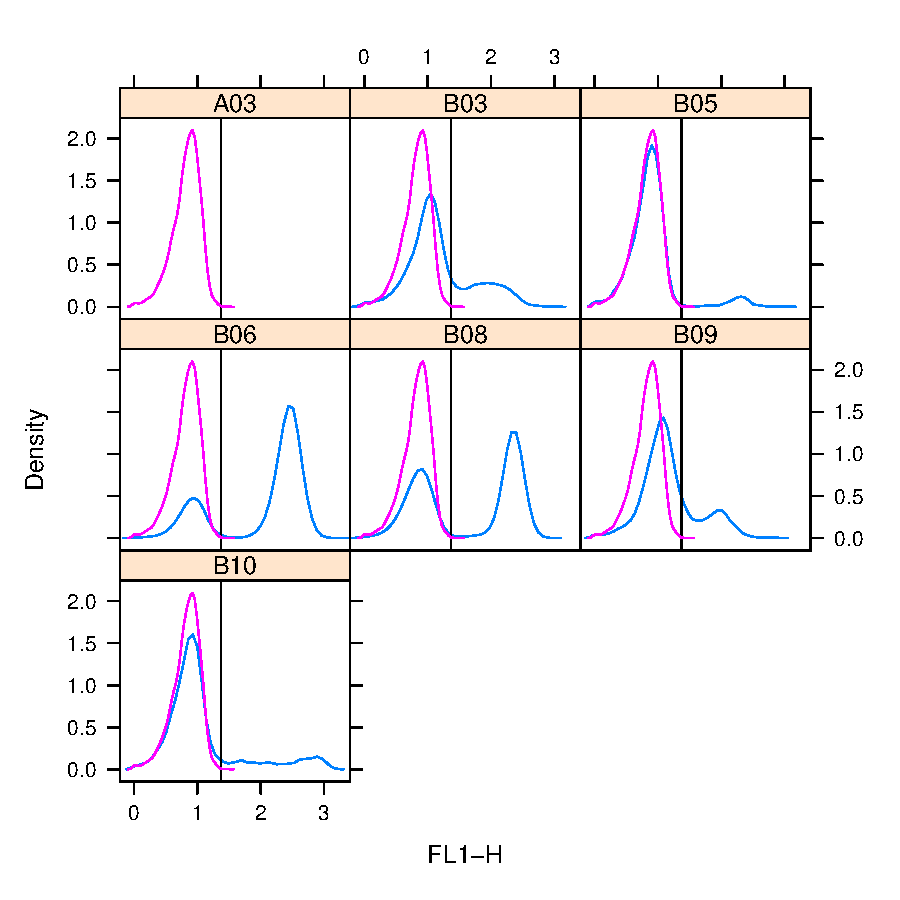
\includegraphics{outline-isoGate}
\caption{Density plots for the A03 isotype well and the associated test wells. Isotype results are shown in magenta while the test samples
are in blue. The vertical bar indicates the negative control gate, estimated using the setControlGates function with numMads=6. This
plot was created using the densityplot function specific to \Robject{flowPlates} from \Rpackage{plateCore}.}
\label{fig:isoGate}
\end{figure}

\clearpage
The wellAnnotation \Robject{data.frame} associated with each analyzed \Robject{flowPlate} can then be exported from R for
use in other programs. Sample output for well B10 in this analysis is given in Table~\ref{tab:wellAnno}. Threshold
gates created using the isotype control wells are included in the \emph{Negative.Control.Gate} column, allowing the gating to be replicated on other
software platforms.

\begin{table}[ht]
\begin{center}
\begin{tabular}{r|ccc}
  \hline
Column & B10 FL2-H &  B10 FL1-H & B10 FL4-H \\
    \hline
  Well.Id & B10 & B10 & B10 \\
  Sample.Type & Test & Test & Test \\
  Ab.Name & Cdbd28 & Cdbd29 & Cdbd30 \\
  Channel & FL2-H & FL1-H & FL4-H \\
  Negative.Control & A03 & A03 & A03 \\
  plateName & PBMC.001 & PBMC.001 & PBMC.001 \\
  name & 0877408774.B10 & 0877408774.B10 & 0877408774.B10 \\
  Negative.Control.Gate & 24 & 23 & 68 \\
  Percent.Positive &  1 & 15 &  0 \\
  Total.Count & 7598 & 7598 & 7598 \\
  Positive.Count &   58 & 1187 &    6 \\
  MFI &  4.0 &  8.2 & 11.8 \\
  MFI.Ratio & 0.64 & 1.14 & 0.78 \\
   \hline
\end{tabular}
\caption{Output for well B10 from the wellAnnotation \Robject{data.frame} associated with the PBMC \Robject{flowPlate}.}
\label{tab:wellAnno}
\end{center}
\end{table}

%%%%%%%%%%%%%%%%%%%%%%%%%%%%%%%%%%%%%%%%%%%%%%%%%%%%%%%%%%%%%%%%%%%%%%%%%%%%%%%%%%%%%%%%%%%%%%%%%%%%%%%%%%%%%%%%%%%%%%%%%%%%%%%%%%%
\clearpage
\section*{Results}
\subsection*{\Rpackage{plateCore} Output}

FCM files from 5 PBMC plates that had been analyzed using BD FACS$^{\text{TM}}$ CAP were processed using the method
described in the analysis section. The resulting \Robject{flowPlates} were stored in \emph{RData} files so that individual plots
can be made without rerunning the analysis. The \Robject{wellAnnotation} for each \Robject{flowPlate} was then merged
into a single \Robject{data.frame}, containing the percent positive results from each plate. These values can then visualized
using microarray tools in R (Figure~\ref{fig:pbmcHeat}). 

Once a marker of interest has been identified, the next step is usually to make density or dotplots of the signals from each
plate. Although these plots can be created individually, it is more convenient to have a combined data object so that results 
from multiple \Robject{flowPlates} can be quickly summarized. \Rpackage{plateCore} supports combining \Robject{flowPlates} using
the \Rfunction{fpbind} function. 
\begin{Schunk}
\begin{Sinput}
> virtPlate <- fpbind(plate1,plate2,plate3,plate4,plate5)
\end{Sinput}
\end{Schunk}
This virtual plate can then be used to make histograms for particular markers, such as CDbd69 which showed variable levels of
expression between the different donors (Figure~\ref{fig:pbmcCDbd69}). 
\begin{Schunk}
\begin{Sinput}
> densityplot(~ `FL2-H` | as.factor(plateName),
+ 	virtPlate,filterResult="Negative.Control")
\end{Sinput}
\end{Schunk}

\begin{figure}
\centering
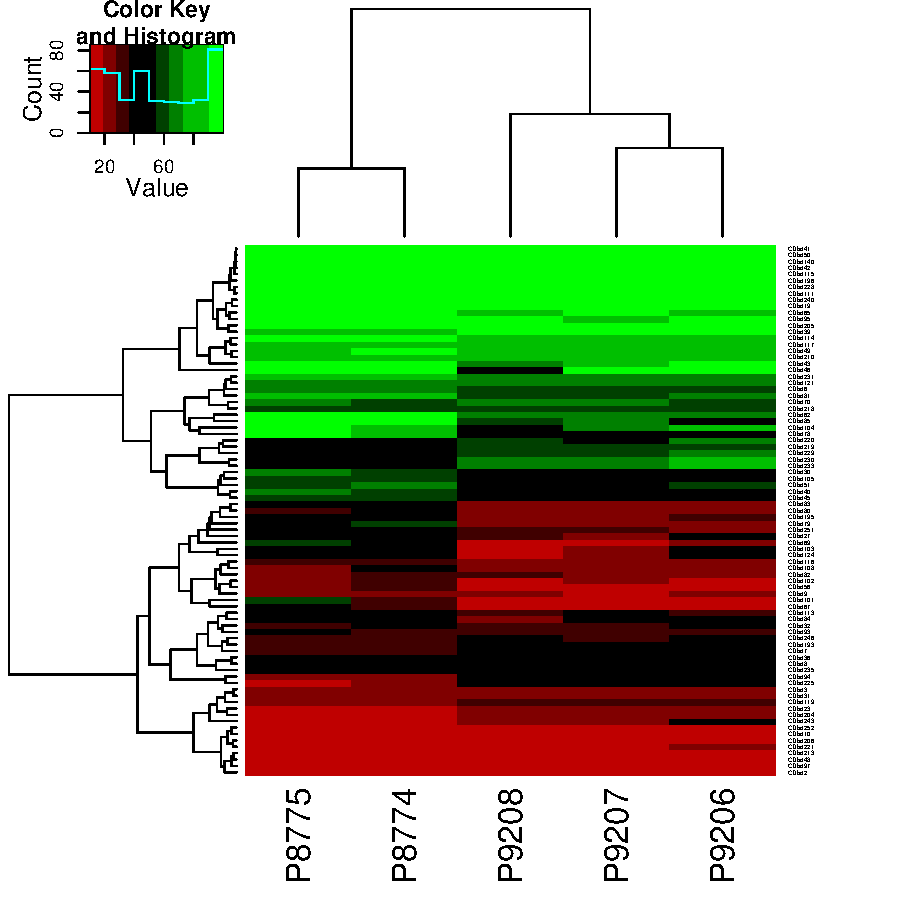
\includegraphics{outline-pbmcHeat}
\caption{Heatmap showing the percentage of positive cells from the 5 different PBMC lymphocyte plates. Only the 83 markers
that had $\ge$ 10\% positive cells are shown here.}
\label{fig:pbmcHeat}
\end{figure}

\begin{figure}
\centering
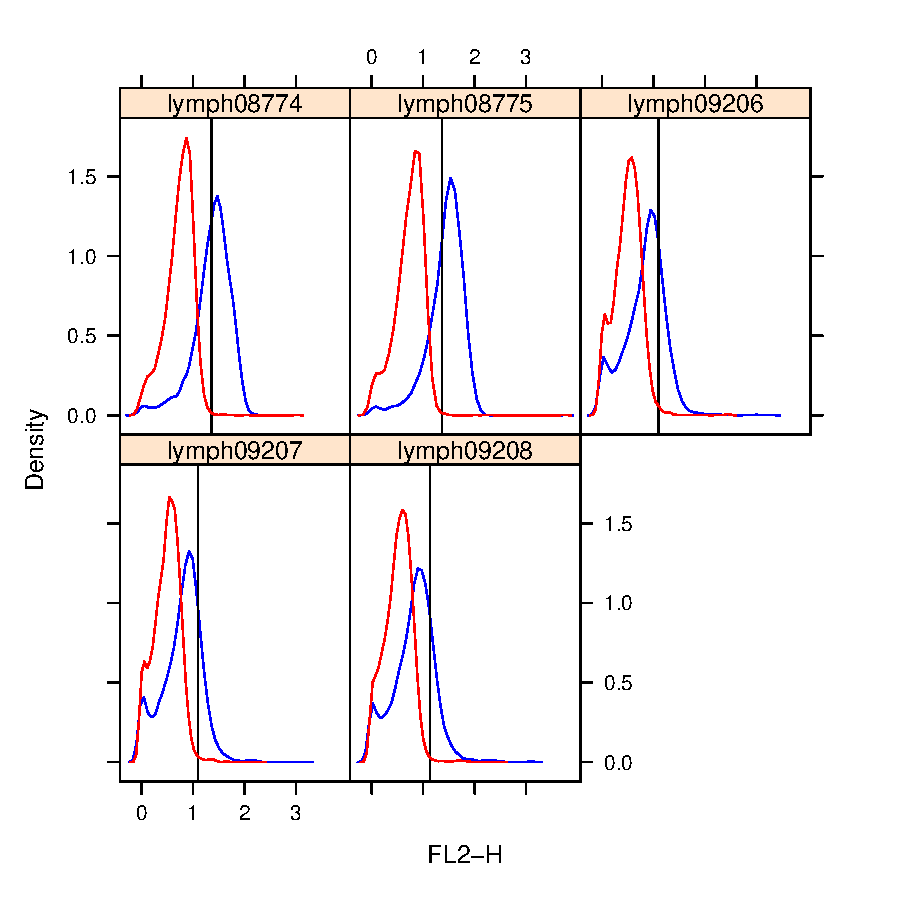
\includegraphics{outline-pbmcCDbd69}
\caption{Dotplots for CDbd69, which is differentially expressed between the 5 PBMC plates. Isotypes are shown in green and
test wells are in magenta.}
\label{fig:pbmcCDbd69}
\end{figure}

%%%%%%%%%%%%%%%%%%%%%%%%%%%%%%%%%%%%%%%%%%%%%%%%%%%%%%%%%%%%%%%%%%%%%%%%%%%%%%%%%%%%%%%%%%%%%%%%%%%%%%%%%%%%%%%%%%%%%%%%%%%%%%%%%%%
\clearpage
\subsection*{Comparison to Manual Analysis}

The 5 pmbc plates were also analyzed using FlowJo$^{\text{TM}}$, which is one of the standard FCM data analysis platforms.
BD FACS$^{\text{TM}}$ CAP is designed as a screening tool to help identify markers for additional analysis. Since it is 
not practical to have controls specific to each of the 189 antibody-dye conjugates, isotypes were chosen according to the
most common antibody subtypes. Cytometry experts initially set gates according to the isotype controls, and then move the
gates based on positive and negative test samples. Figure~\ref{fig:pcVSman} shows how the results from FlowJo$^{\text{TM}}$ compare to \Rpackage{plateCore}.

\begin{figure}
\centering
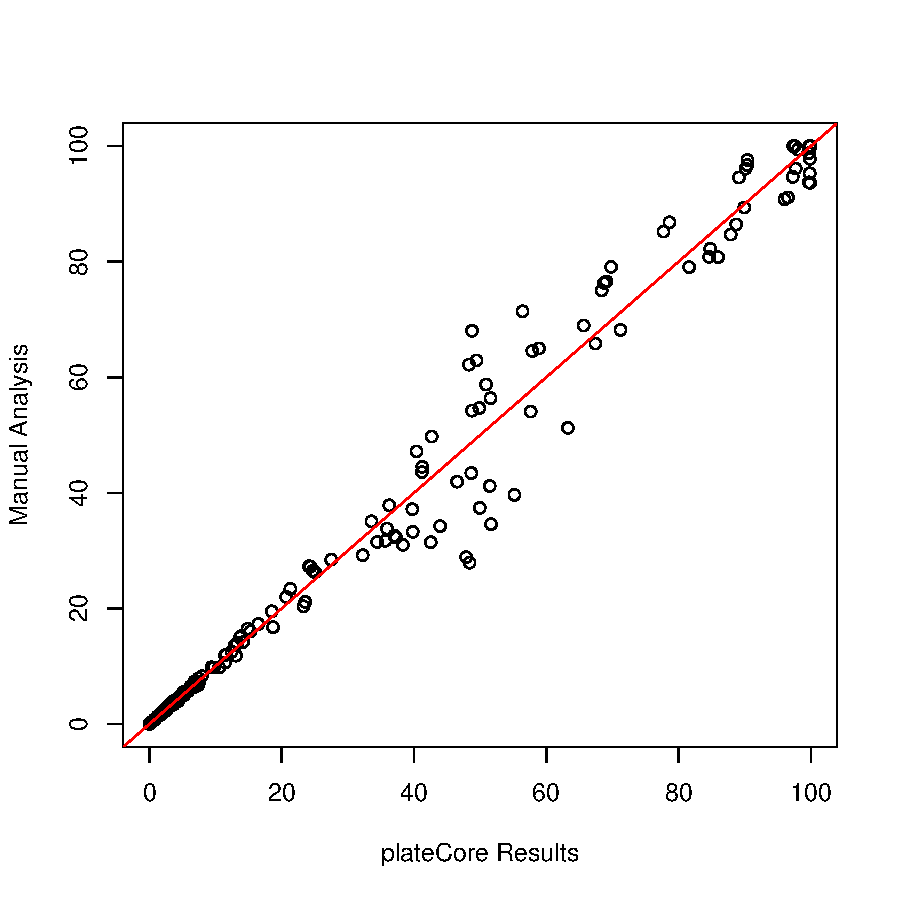
\includegraphics{outline-pcVSman}
\caption{Percent positive results for 189 markers analyzed using either \Rpackage{plateCore} or manually using FlowJo$^{\text{TM}}$. (Note: Need to get real
data in this plot)}
\label{fig:pcVSman}
\end{figure}

%%%%%%%%%%%%%%%%%%%%%%%%%%%%%%%%%%%%%%%%%%%%%%%%%%%%%%%%%%%%%%%%%%%%%%%%%%%%%%%%%%%%%%%%%%%%%%%%%%%%%%%%%%%%%%%%%%%%%%%%%%%%%%%%%%%
\clearpage
\section*{Discussion}

The PBMC example shows that a complex analysis of a 96-well plate, stained with 189 antibodies,
can be constructed in 15-20 lines of code using \Rpackage{plateCore}. Lymphocytes were selected
using \Rpackage{flowCore} gates and visualized using \Rpackage{flowViz} plots. One-dimensional 
gates were constructed using isotype wells and applied to the test wells to identify positive cells.

Given a \textit{plate configuration} file, this same approach can be used to analyze any
negative control based FC-HCS study. Although adjustments to the automatically generated negative control gates may be needed,
these changes change be incorporated into the analysis script and reproduced at a later time.

(Need some additional paragraphs about why plateCore is wonderful).

%%%%%%%%%%%%%%%%%%%%%%%%%%%%%%%%%%%%%%%%%%%%%%%%%%%%%%%%%%%%%%%%%%%%%%%%%%%%%%%%%%%%%%%%%%%%%%%%%%%%%%%%%%%%%%%%%%%%%%%%%%%%%%%%%%%
\section*{References/Recent Related Publications}
\begin{itemize}
\item flowCore manuscript in Cytometry A\\
Gives an overview of flowCore data structures, transformation and gating examples, quality control checks (flowQ), and 
flowCore analysis philosophy.\\
\item Using flowViz to Visualize Flow Cytometry Data, Bioinformatics\\
Uses flowViz to make xyplots, ecdfplots, and time plots of GvHD data. Makes the case that visualizations can be used to aid automation.
\item Quality Assessment of Ungated Flow Cytometry data in High Throughput experiments, Cytometry A, GvHD data\\
Visualizing data: xyplots, histograms, ecdfplots, boxplots, and contour plots.\\
Outlier detection (Grubbs and KS)\\
Using flowViz/Core graphical output for quality assessment\\
\item Analysis of flow cytometry data using an automatic processing tool, Cytometry Part A\\
Automated analysis in Matlab.\\
\end{itemize}


\end{document}
